\documentclass[a4paper]{article} 
\usepackage{graphicx} 
\usepackage[ngerman]{babel} 
\usepackage[ansinew]{inputenc} 
\usepackage[T1]{fontenc} 
\usepackage{tgpagella} 
\usepackage{geometry} 
\usepackage{color} 
\usepackage{microtype} 
\usepackage{minted}
\usepackage{caption}
\usepackage[headsepline,footsepline]{scrpage2}
\usepackage{textcomp}
\usepackage{pdfpages}
\usepackage{mdframed}



\makeatletter
\renewcommand\minted@pygmentize[2][\jobname.pyg]{
  \def\minted@cmd{pygmentize -l #2 -f latex -F tokenmerge
    \minted@opt{gobble} \minted@opt{texcl} \minted@opt{mathescape}
    \minted@opt{startinline} \minted@opt{funcnamehighlighting}
    \minted@opt{linenos} -P "verboptions=\minted@opt{extra}"
    -O encoding=UTF-8,outencoding=iso-8859-1 -o \jobname.out.pyg #1}
  \immediate\write18{\minted@cmd}
  % For debugging, uncomment:
  %\immediate\typeout{\minted@cmd}
  \ifthenelse{\equal{\minted@opt@bgcolor}{}}
   {}
   {\begin{minted@colorbg}{\minted@opt@bgcolor}}
  \input{\jobname.out.pyg}
  \ifthenelse{\equal{\minted@opt@bgcolor}{}}
   {}
   {\end{minted@colorbg}}
  \DeleteFile{\jobname.out.pyg}}
\makeatother


\title{Dokumentation - 6 Übung}
\author{Roman Lumetsberger}
\date{\today}

\newmintedfile[ccode]{cpp}{
               linenos,
               numbersep=5pt,
               frame=lines,
               framesep=2mm
}

\newmintedfile[javacode]{java}{
               linenos,
               numbersep=5pt,
               frame=lines,
               tabsize=2,
               framesep=2mm,
}
\newmintedfile[csscode]{css}{
               linenos,
               numbersep=5pt,
               frame=lines,
               tabsize=2,
               framesep=2mm,
}
\newmintedfile[sqlcode]{sql}{
               linenos,
               numbersep=5pt,
               frame=lines,
               tabsize=2,
               framesep=2mm,
}
\captionsetup{
  font=footnotesize,
  justification=raggedright,
  singlelinecheck=false
}


\newcommand{\srcDir}{../Beispiel/src/at/lumetsnet/caas/}
\newcommand{\testDir}{../Beispiel/test/at/lumetsnet/caas/test/}

\definecolor{lineColor}{RGB}{151,0,0}
\pagestyle{scrheadings}
\clearscrheadfoot
\begin{document}
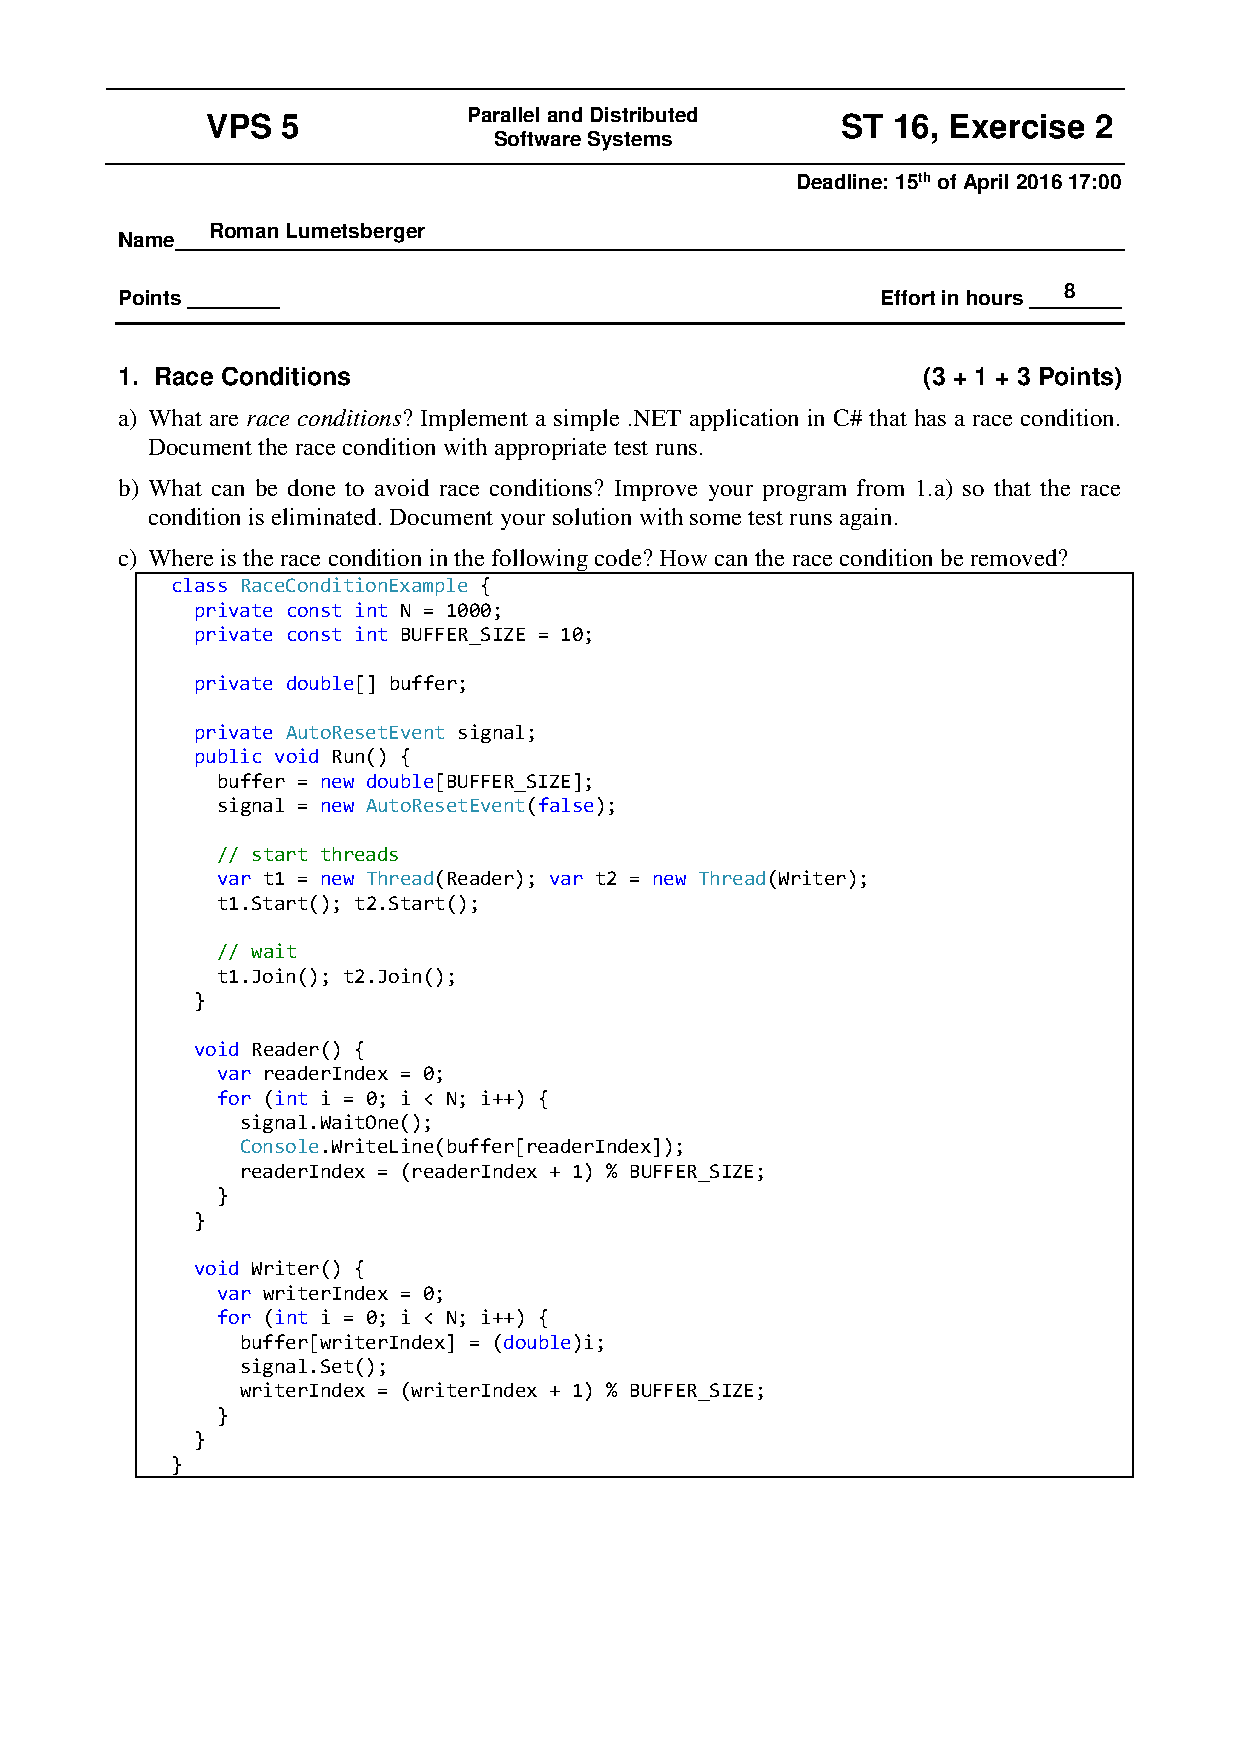
\includepdf[pages=-]{angabe.pdf}

\ihead{VPS SS 2016 - �bung 02}
\ifoot{Roman Lumetsberger}
\cfoot{1310307026}
\ofoot{Seite \pagemark}

\section{Race Conditions}
\subsection*{1a. Was sind race conditions?}
\textbf{Race conditions} treten bei Programmen auf, bei denen die Ergebnisse von der zeitlichen Abfolge der Threads abh�ngig und somit nicht vorhersehbar sind. Sie k�nnen entstehen, wenn mehrere Threads parallel auf den selben Speicherbereich (Variable) zugreifen und ver�ndern.

\begin{figure}[!htb]
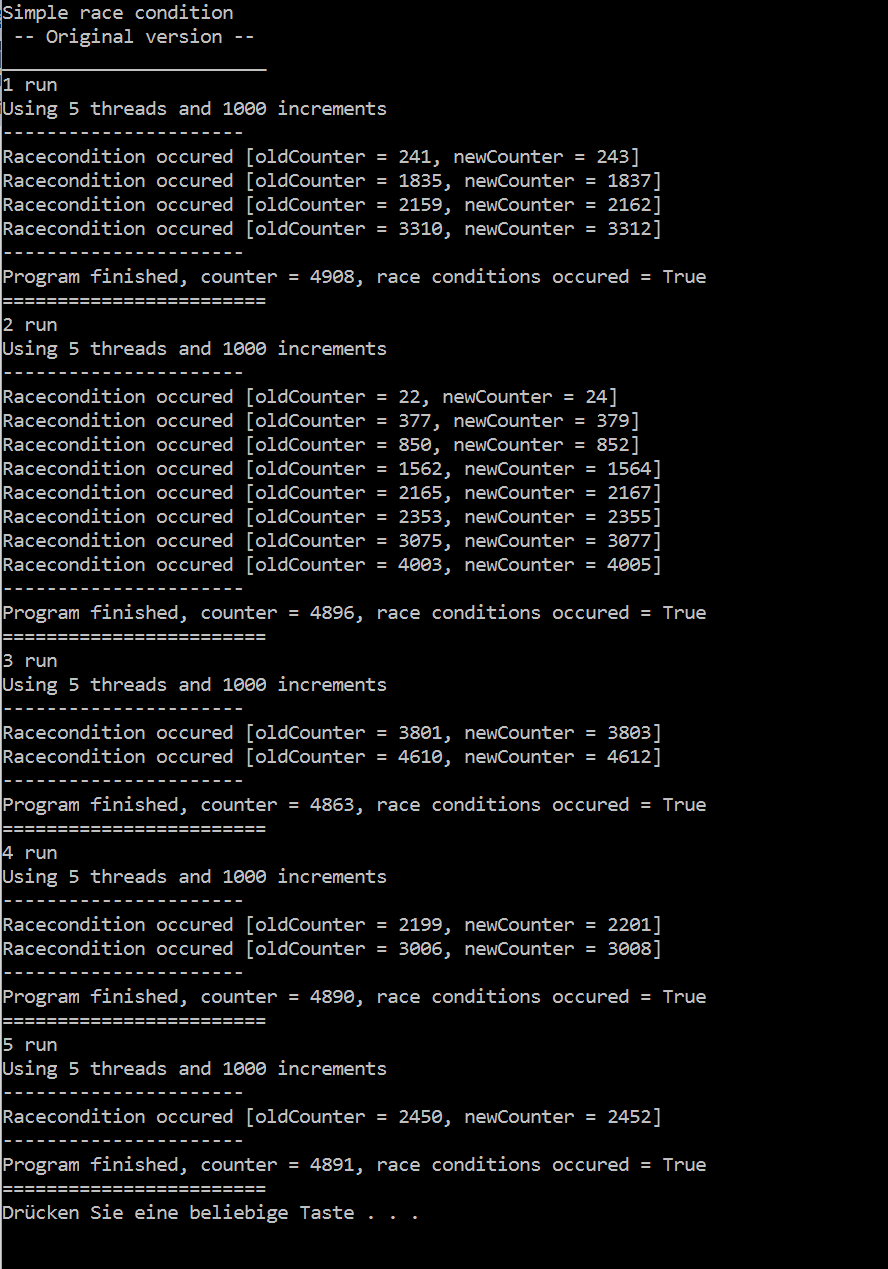
\includegraphics[width=300px]{images/1a.png}
\caption{Race condition in CSharp - Original version}
\label{fig:SimpleRaceConditionOriginal}
\end{figure}

Abbildung~\ref{fig:SimpleRaceConditionOriginal} zeigt die Ausgabe der implementierten race codition in CSharp. Dabei wird eine Variable \texttt{\_counter} in der Methode \texttt{ThreadMethod} erh�ht und dann mit dem vorherigen Wert verglichen. Diese Methode wird dann paralell von mehreren Threads verwendet. Der neue Wert sollte genau um eins gr��er sein als der alte Wert. Ist dies nicht der Fall ist eine race condition aufgetreten. Die Variable wurde also von einem anderen Thread �berschrieben.

\emph{Soucecode siehe 1b. mit Parameter \texttt{useLock = false} }

\subsection*{1b. Wie k�nnen race conditions vermieden werden?}
Diese k�nnen mit Hilfe von Locks vermieden werden.
\begin{figure}[!htb]
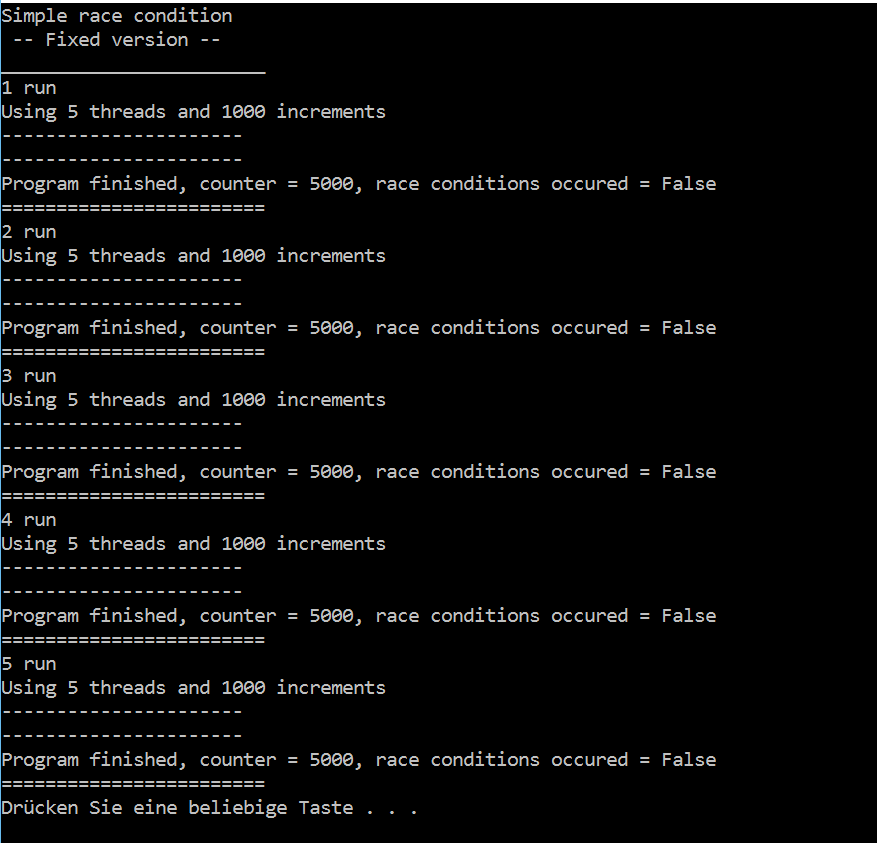
\includegraphics[width=300px]{images/1b.png}
\caption{Race condition in CSharp - Ohne race condition}
\label{fig:SimpleRaceConditionFixed}
\end{figure}

Abbildung~\ref{fig:SimpleRaceConditionFixed} zeigt die Ausgabe der verbesserten Version. Diese verwendet Locks um die race condition zu vermeiden.

\subsubsection*{1a./1b. Sourccode (Code/SimpleRaceCondition)}
\emph{Soucecode mit Parameter \texttt{useLock = true} }
\cscode{\srcDir/SimpleRaceCondition/SimpleRaceCondition.cs}

\subsection*{1c. Race condition im Code}
Die race condition im angegebenen Code ist die Tatsache, dass der Writer und Reader nicht korrekt miteinander synchronisiert sind und nur ein begrenzter Puffer zur Verf�gung steht. Dadurch kann es sein, dass der Writer bereits mehr Werte erzeugt als der Puffer zul�sst und somit die alten Werte �berschreibt.
Die L�sung ist die korrekte Synchronisation der beiden Threads mit Hilfe von zwei Semaphoren. Die \texttt{writerSemaphore} wird auf die \texttt{BUFFER\_SIZE} initialisiert und kann somit diese Anzahl an Elementen schreiben, bevor sie warten muss, bis der \texttt{Reader} die Werte ausgegeben hat.	
\subsubsection*{1c. Sourccode (Code/RaceConditionExample)}
\cscode{\srcDir/RaceConditionExample/RaceConditionExample.cs}

\section{Synchronization Primitives}
\subsection*{2a. / 2b.}

\subsubsection*{2a.}
Um nur 10 Dateien parallel herunterzuladen, kann eine Semaphore verwendet werden, die die gleichzeitige Anzahl an Downloads auf maximal 10 begrenzt. Dazu wird die Variable \texttt{\_syncSemaphore} eingef�hrt und mit dem Wert 10 initialisiert. In der Methode \texttt{DownloadFile} wird dann \texttt{\_syncSemaphore.Wait()} verwendet, um die Downloads zu begrenzen. Wenn ein Download fertig ist, wird die Semaphore wieder freigegeben \texttt{\_syncSemaphore.Release()}.

\subsubsection*{2b.}
Um auf alle Threads zu warten, m�ssen diese in einer Liste gespeichert und dann f�r jeden die Methode \texttt{Join} aufgerufen werden.

\subsubsection*{2a./2b. Sourccode (Code/SynchronizationPrimitives)}
\cscode{\srcDir/SynchronizationPrimitives/LimitedConnectionsExample.cs}

\subsection*{2c. Aktives Warten}
Um das Polling zu verhindern, k�nnen alle Tasks in einer Liste gespeichert und dann mit der Methode \texttt{Task.WaitAll} auf alle gewartet werden.
\subsubsection*{2.c Sourccode (Code/SynchronizationPrimitives)}
\cscode{\srcDir/SynchronizationPrimitives/PollingExample.cs}

\section{Toilet Simulation}
\subsection*{3a. Toilet Implementierung}
Diese Aufgabe wurde bereits in der �bung implementiert. Der \texttt{Consumer} ist fertig, wenn alle Elemente der Warteschlange abgearbeitet sind. Dazu wurde das Interface \texttt{IQueue} um das Property \texttt{IsCompleted} erweitert.

Die Synchronisation wurde ebenfalls �ber die Warteschlange gel�st. Hier wurde das Interface \texttt{IQueue} um die Methode \texttt{TryDequeue} erweitert. Diese blockiert, falls aktuell kein Element vorhanden ist, aber noch nicht alle Elemente hinzugef�gt wurden.

\subsection*{3b. FifoQueue Implementierung}
Die \texttt{FifoQueue} wurde mit Hilfe einer Semaphore implementiert. Dabei wird bei jedem \texttt{Enqueue} die Semaphore um Eins erh�ht und beim \texttt{TryDequeue} wird diese wieder veringert. Damit wird der gew�nschte Effekt erreicht, das die Methode \texttt{TryDequeue} blockiert. Dabei kann es vorkommen, dass die Queue bereits leer ist und trotzdem noch Threads in der Methode \texttt{TryDequeue} auf Elemente warten. Um das Warten zu beenden, wurde ein \texttt{CancellationToken} verwendet, der beim \texttt{Wait} mitgegeben wird. Damit k�nnen diese Threads aufgeweckt und beendet werden. Um race conditions zu vermeiden, wurde jeder Zugriff auf den Datenspeicher mit Locks gesch�tzt.

\subsubsection*{3b. Sourcecode (Code/ToiletSimulationForStudents)}
\cscode{\srcDir/ToiletSimulationForStudents/Queue.cs}
\cscode{\srcDir/ToiletSimulationForStudents/FIFOQueue.cs}

\pagebreak
\subsubsection*{Parameter}
\begin{itemize}
\item Producers: 2
\item Jobs per produce: 200
\item Consumers: 2
\item Mean Arrival Time: 100ms
\item Mean Due Time: 500ms
\item Std. Dev. Due Time: 150ms
\item Mean Processing Time: 100ms
\item Std. Dev. Processing Time: 25ms
\end{itemize}

\subsubsection*{Ergebnisse}
\begin{table}[!htb]
\centering
\caption{Ergebnisse FifoQueue}
\label{3berg}
\begin{tabular}{llrll}
\hline
\multicolumn{5}{c}{Simulation} \\ \cline{1-5}                                                                                 
Lauf & \begin{tabular}[c]{@{}l@{}}Nicht erfolgreiche\\ Jobs\end{tabular} & Verh�ltnis & Wartezeit     & � Wartezeit  \\ \cline{1-5}
1    & 222                                                               & 0,555      & 00:03:07.4319 & 00:00:00.469 \\
2    & 67                                                                & 0,168      & 00:01:18.8208 & 00:00:00.167 \\
3    & 142                                                               & 0,356      & 00:02:13.6162 & 00:00:00.334 \\
4    & 239                                                               & 0,598      & 00:05:04.3024 & 00:00:00.761 \\
5    & 310                                                               & 0,775      & 00:07:09:1210 & 00:00:01.073 \\ \cline{1-5}
\textbf{�}    & \textbf{196}                                                               & \textbf{0,490}      & 00:03:45.450 & \textbf{00:00:00.530} \\
Std. Abw.    & 83,750                                                               & 0,2092      & 00:02:05.926 & 00:00:00.361 \\ \cline{1-5}

\end{tabular}
\end{table} 

\subsection*{3c. ToiletQueue Implementierung}
Um die Abarbeitung der Jobs zu verbessern, kann der n�chste Job anhand der Endzeit und Arbeitszeit ausgew�hlt werden. Dabei k�nnen die Jobs anhand der sp�testen Startzeit ( = Endzeit - Arbeitszeit) sortiert und dann der erste Eintrag der Liste verwendet werden. Als zus�tzliche Optimierung k�nnen dann noch jene Jobs, bei denen die sp�teste Startzeit bereits in der Vergangenheit liegt, hinten angestellt werden (bei diesen Jobs ist es sowieso schon zu sp�t).

Um die Implementierung zu vereinfachen, wurden das Interface \texttt{IJob} um das Property \texttt{LatestStartTime} erweitert und in \texttt{Person} implementiert. Die \texttt{ToiletQueue} selbst stellt eine Ableitung der \texttt{FiFoQueue} und �berschreibt die Methode \texttt{GetNextJob}. Diese Methode w�hlt dann den n�chsten Job anhand des oben angef�hrten Algorithmus aus.

\subsubsection*{3c. Sourcecode (Code/ToiletSimulationForStudents)}
\cscode{\srcDir/ToiletSimulationForStudents/ToiletQueue.cs}


\subsubsection*{Parameter}
\begin{itemize}
\item Producers: 2
\item Jobs per produce: 200
\item Consumers: 2
\item Mean Arrival Time: 100ms
\item Mean Due Time: 500ms
\item Std. Dev. Due Time: 150ms
\item Mean Processing Time: 100ms
\item Std. Dev. Processing Time: 25ms
\end{itemize}

\subsubsection*{Ergebnisse}

\begin{table}[!htb]
\centering
\caption{Ergebnisse ToiletQueue}
\label{3berg}
\begin{tabular}{llrll}
\hline
\multicolumn{5}{c}{Simulation} \\ \cline{1-5}
Lauf & \begin{tabular}[c]{@{}l@{}}Nicht erfolgreiche\\ Jobs\end{tabular} & Verh�ltnis & Wartezeit     & � Wartezeit  \\ \cline{1-5}
1    & 35                                                               & 0,0875      & 00:05:11.0704 & 00:00:00.469 \\
2    & 30                                                                & 0,075      & 00:03:40.0223 & 00:00:00.550 \\
3    & 41                                                                & 0,103      & 00:05:58.6884 & 00:00:00.103 \\
4    & 40                                                               & 0,100       & 00:05:30.3139 & 00:00:00.826 \\
5    & 37                                                               & 0,093      & 00:06:07:2078 & 00:00:00.918 \\ \cline{1-5}
\textbf{�}    & \textbf{36,6}     	                                                          & \textbf{0,091}      & 00:05:17.461 & \textbf{00:00:00.573} \\
Std. Abw.    & 3,029                                                               & 0,00995      & 00:00:52.678 & 00:00:00.288 \\ \cline{1-5}

\end{tabular}
\end{table} 

\subsubsection*{Vergleich}

Die Durchschnittliche Anzahl an nicht rechtzeitig abgearbeiteten Jobs hat sich von 196 auf 36 reduziert und dadurch k�nnen mehr Kunden zufriedengestellt werden. Weiters hat sich das Verh�ltnis auf 0,49 auf 0,091 reduziert. Obwohl die Reihenfolge der Jobs anders ist, ist die durchschnittliche Wartezeit nahezu gleich geblieben. 
\end{document}